\section{Введение}
Проведение прямых измерений физических величин является основой любого экспериментального исследования. Для получения достоверных результатов необходимо не только использовать точное оборудование, но и владеть методами математической статистики для корректной оценки погрешностей. Данная работа посвящена освоению этих навыков на примере анализа временных характеристик импульсного сигнала


\subsection{Цель работы}

Ознакомиться с методикой прямых многократных измерений физических величин на примере измерения периода следования импульсов с помощью электронного частотомера. Провести статистическую обработку выборки экспериментальных данных, оценить погрешности и построить графики распределения. 


\subsection{Решаемые задачи}
\begin{enumerate}
    \item Провести измерения периода на грубой и точной шкалах частотомера.
    \item Реализовать алгоритмы статистической обработки (без использования стандартных библиотек) для вычисления среднего, дисперсии и доверительного интервала.
    \item Построить график временного дрейфа и гистограмму распределения.
\end{enumerate}

\section{Основная часть}

\subsection{Теоретическая часть}
В работе используются методы математической статистики для обработки прямых измерений. Наилучшей оценкой истинного значения является среднее арифметическое:
\begin{equation}
    \bar{T} = \frac{1}{n}\sum_{i=1}^{n} T_i
\end{equation}
Для оценки разброса используется несмещенная оценка дисперсии и стандартное отклонение отдельного измерения:
\begin{equation}
    S_T = \sqrt{\frac{1}{n-1}\sum_{i=1}^{n} (T_i - \bar{T})^2}
\end{equation}
Случайная погрешность (доверительный интервал) для среднего значения рассчитывается с использованием коэффициента Стьюдента $t_{\alpha, n}$:
\begin{equation}
    \Delta T_{sl} = t_{\alpha, n} \cdot \frac{S_T}{\sqrt{n}}
\end{equation}
%Полная погрешность определяется с учетом приборной погрешности $\Delta T_{prib}$:
%\begin{equation}
%    \Delta T_{poln} = \sqrt{\Delta T_{sl}^2 + \left(\frac{\Delta T_{prib}}{3}\right)^2}
%\end{equation}


\subsection{Эксперимент}
Измерения проводились с помощью установки, состоящей из генератора импульсов (задающего сигнал) и электронного частотомера Ч3-32. На частотомер подавалась последовательность импульсов, период которых измерялся сначала на грубой шкале, а затем, для получения статистической выборки из n=50 значений, — на точной

\begin{figure}[H]
\centering
\includegraphics[width=0.8\textwidth]{Device.jpg} 
\caption{Фотография используемой измерительной установки}
\label{fig:device}
\end{figure}

\subsection{Обработка данных и обсуждение результатов}

\subsubsection{Исходный код}
Все алгоритмы (расчет среднего, дисперсии, стандартного отклонения) были реализованы самостоятельно на языке Python. Исходный код загружен в репозиторий GitHub по адресу: \url{https://github.com/st128113/Workshop1}.

%\begin{lstlisting}[language=Python, caption=Функция расчета дисперсии без сторонних библиотек]
%def calc_variance(arr, mean):
%    s = 0.0
%    for x in arr:
%        s += (x - mean)**2
%    return s / (len(arr) - 1)
%\end{lstlisting}

\subsubsection{Таблицы}
\subsubsection{Таблицы}

Ниже представлены результаты измерений периода следования импульсов на грубой и точной шкалах частотомера, а также промежуточные расчеты для вычисления дисперсии.

% ================= ТАБЛИЦА 1 (Грубая шкала) =================
\begin{table}[H]
\centering
\caption{Результаты измерений на грубой шкале}
\label{tabl:1}
\begin{tabular}{|c|c|c|c|}
\hline
\begin{minipage}{10mm} \centering № \\ п.п. \end{minipage} &
\begin{minipage}{4cm} \centering Диапазон \\ показаний шкалы \end{minipage} &
\begin{minipage}{4cm} \centering Результат \\ наблюдения ($T_i$) \end{minipage} &
\begin{minipage}{4cm} \centering Погрешность \\ прибора ($\Delta T_{\text{приб}}$) \end{minipage} \\
\hline
 & с & мс & мс \\
\hline
1  & $10^{-4}$ & 274.1 & 0.1 \\
2  & $10^{-4}$ & 274.3 & 0.1 \\
3  & $10^{-4}$ & 273.7 & 0.1 \\
4  & $10^{-4}$ & 273.9 & 0.1 \\
5  & $10^{-4}$ & 274.0 & 0.1 \\
6  & $10^{-4}$ & 273.6 & 0.1 \\
7  & $10^{-4}$ & 274.4 & 0.1 \\
8  & $10^{-4}$ & 274.2 & 0.1 \\
9  & $10^{-4}$ & 274.0 & 0.1 \\
10 & $10^{-4}$ & 274.1 & 0.1 \\
\hline
\multicolumn{4}{|c|}{ $\bar{T} = 274.03$ мс, $\quad \sigma = 0.25$ мс } \\
\hline
\end{tabular}
\end{table}

% ================= ТАБЛИЦА 2 (Точная шкала на 50 значений) =================
\begin{table}[H]
\centering
\caption{Результаты измерений на точной шкале ($\Delta T_{\text{приб}} = 0.001$ мс)}
\label{tabl:2}
\vspace{2mm}
% Делаем таблицу из двух половинок, чтобы влезла на лист
\begin{tabular}{|c|c|c|c||c|c|c|c|}
\hline
№ & $T_i$, мс & $d_i = T_i - \bar{T}$, мс & $d_i^2$, $\text{мс}^2$ & № & $T_i$, мс & $d_i = T_i - \bar{T}$, мс & $d_i^2$, $\text{мс}^2$ \\
\hline
1 & 274.773 & 0.183 & 0.033489 & 26 & 274.464 & -0.126 & 0.015876 \\
2 & 274.673 & 0.083 & 0.006889 & 27 & 274.627 & 0.037 & 0.001369 \\
3 & 274.244 & -0.346 & 0.119716 & 28 & 274.313 & -0.277 & 0.076729 \\
4 & 274.546 & -0.044 & 0.001936 & 29 & 274.412 & -0.178 & 0.031684 \\
5 & 274.580 & -0.010 & 0.000100 & 30 & 274.442 & -0.148 & 0.021904 \\
6 & 274.469 & -0.121 & 0.014641 & 31 & 274.473 & -0.117 & 0.013689 \\
7 & 274.543 & -0.047 & 0.002209 & 32 & 274.457 & -0.133 & 0.017689 \\
8 & 274.599 & 0.009 & 0.000081 & 33 & 274.381 & -0.209 & 0.043681 \\
9 & 274.127 & -0.463 & 0.214369 & 34 & 274.235 & -0.355 & 0.126025 \\
10 & 274.345 & -0.245 & 0.060025 & 35 & 274.584 & -0.006 & 0.000036 \\
11 & 274.601 & 0.011 & 0.000121 & 36 & 274.882 & 0.292 & 0.085264 \\
12 & 274.440 & -0.150 & 0.022500 & 37 & 274.819 & 0.229 & 0.052441 \\
13 & 274.452 & -0.138 & 0.019044 & 38 & 274.510 & -0.080 & 0.006400 \\
14 & 274.278 & -0.312 & 0.097344 & 39 & 274.872 & 0.282 & 0.079524 \\
15 & 274.614 & 0.024 & 0.000576 & 40 & 274.648 & 0.058 & 0.003364 \\
16 & 274.470 & -0.120 & 0.014400 & 41 & 275.020 & 0.430 & 0.184900 \\
17 & 274.790 & 0.200 & 0.040000 & 42 & 274.481 & -0.109 & 0.011881 \\
18 & 274.709 & 0.119 & 0.014161 & 43 & 274.539 & -0.051 & 0.002601 \\
19 & 274.660 & 0.070 & 0.004900 & 44 & 274.497 & -0.093 & 0.008649 \\
20 & 274.965 & 0.375 & 0.140625 & 45 & 274.241 & -0.349 & 0.121801 \\
21 & 274.759 & 0.169 & 0.028561 & 46 & 274.925 & 0.335 & 0.112225 \\
22 & 274.639 & 0.049 & 0.002401 & 47 & 274.853 & 0.263 & 0.069169 \\
23 & 274.945 & 0.355 & 0.126025 & 48 & 274.716 & 0.126 & 0.015876 \\
24 & 274.880 & 0.290 & 0.084100 & 49 & 274.653 & 0.063 & 0.003969 \\
25 & 274.684 & 0.094 & 0.008836 & 50 & 274.663 & 0.073 & 0.005329 \\
\hline
\multicolumn{8}{|c|}{ $\bar{T} = 274.590$ мс, $\quad \sum d_i \approx 0$, $\quad \sum d_i^2 = 2.169$ $\text{мс}^2$ } \\
\hline
\end{tabular}
\end{table}

\subsubsection{Графики}
Для более детального анализа построим интервальное распределение результатов измерений. Весь диапазон значений от минимального \(T_{\min}=274.127\) мс до максимального \(T_{\max}=275.020\) мс был разбит на 9 интервалов шириной \(0.12\) мс. Подсчитано число попаданий \(\Delta n\) в каждый интервал и соответствующая доля \(\Delta n/n\) (табл.~\ref{tab:hist_dist}).

\begin{table}[H]
\centering
\caption{Интервальное распределение результатов измерений на точной шкале}
\label{tab:hist_dist}
\begin{tabular}{|c|c|c|c|}
\hline
№ интервала & Границы интервала, мс & Число попаданий \(\Delta n\) & Доля \(\Delta n / n\) \\
\hline
1 & 274.12--274.24 & 2 & 0.040 \\
2 & 274.24--274.36 & 5 & 0.100 \\
3 & 274.36--274.48 & 10 & 0.200 \\
4 & 274.48--274.60 & 9 & 0.180 \\
5 & 274.60--274.72 & 12 & 0.240 \\
6 & 274.72--274.84 & 4 & 0.080 \\
7 & 274.84--274.96 & 6 & 0.120 \\
8 & 274.96--275.08 & 2 & 0.040 \\
9 & 275.08--275.20 & 0 & 0.000 \\
\hline
\end{tabular}
\end{table}

По данным таблицы можно оценить стандартное отклонение графическим методом. Максимальная доля попаданий составляет \(0.240\) в интервале 5. На уровне \(0.6\) от максимума (\(0.6 \times 0.240 = 0.144\)) распределение перекрывает интервалы с 3 по 5, что соответствует ширине примерно \(274.72 - 274.36 = 0.36\) мс. Для нормального распределения такая ширина приблизительно равна \(2\sigma\), следовательно, \(\sigma_{\text{граф}} \approx 0.18\) мс.

Рассчитаем стандартное отклонение по формуле (2):
\[
S_T = \sqrt{\frac{\sum d_i^2}{n-1}} = \sqrt{\frac{2.169}{49}} \approx 0.210\ \text{мс}.
\]
Полученное значение хорошо согласуется с графической оценкой, учитывая приближённость последней.

Далее вычислим стандартную неопределённость среднего:
\[
s_{\bar{T}} = \frac{S_T}{\sqrt{n}} = \frac{0.210}{\sqrt{50}} \approx 0.0297\ \text{мс}.
\]
Для доверительной вероятности \(\alpha = 0.95\) и числа степеней свободы \(n-1 = 49\) коэффициент Стьюдента \(t_{0.95;49} \approx 2.01\). Тогда доверительный интервал:
\[
\Delta T = t_{\alpha,n} \cdot s_{\bar{T}} \approx 2.01 \times 0.0297 \approx 0.060\ \text{мс}.
\]
Инструментальная погрешность частотомера на точной шкале \(\Delta T_{\text{приб}} = 0.001\) мс, что даёт стандартную неопределённость прибора \(u_{\text{приб}} = 0.001/3 \approx 0.0003\) мс. Эта величина пренебрежимо мала по сравнению со случайной составляющей, поэтому полная погрешность определяется только случайной погрешностью. Окончательный результат измерения периода:
\[
T = (274.590 \pm 0.060)\ \text{мс},\quad \alpha = 0.95.
\]

\begin{figure}[H]
\centering
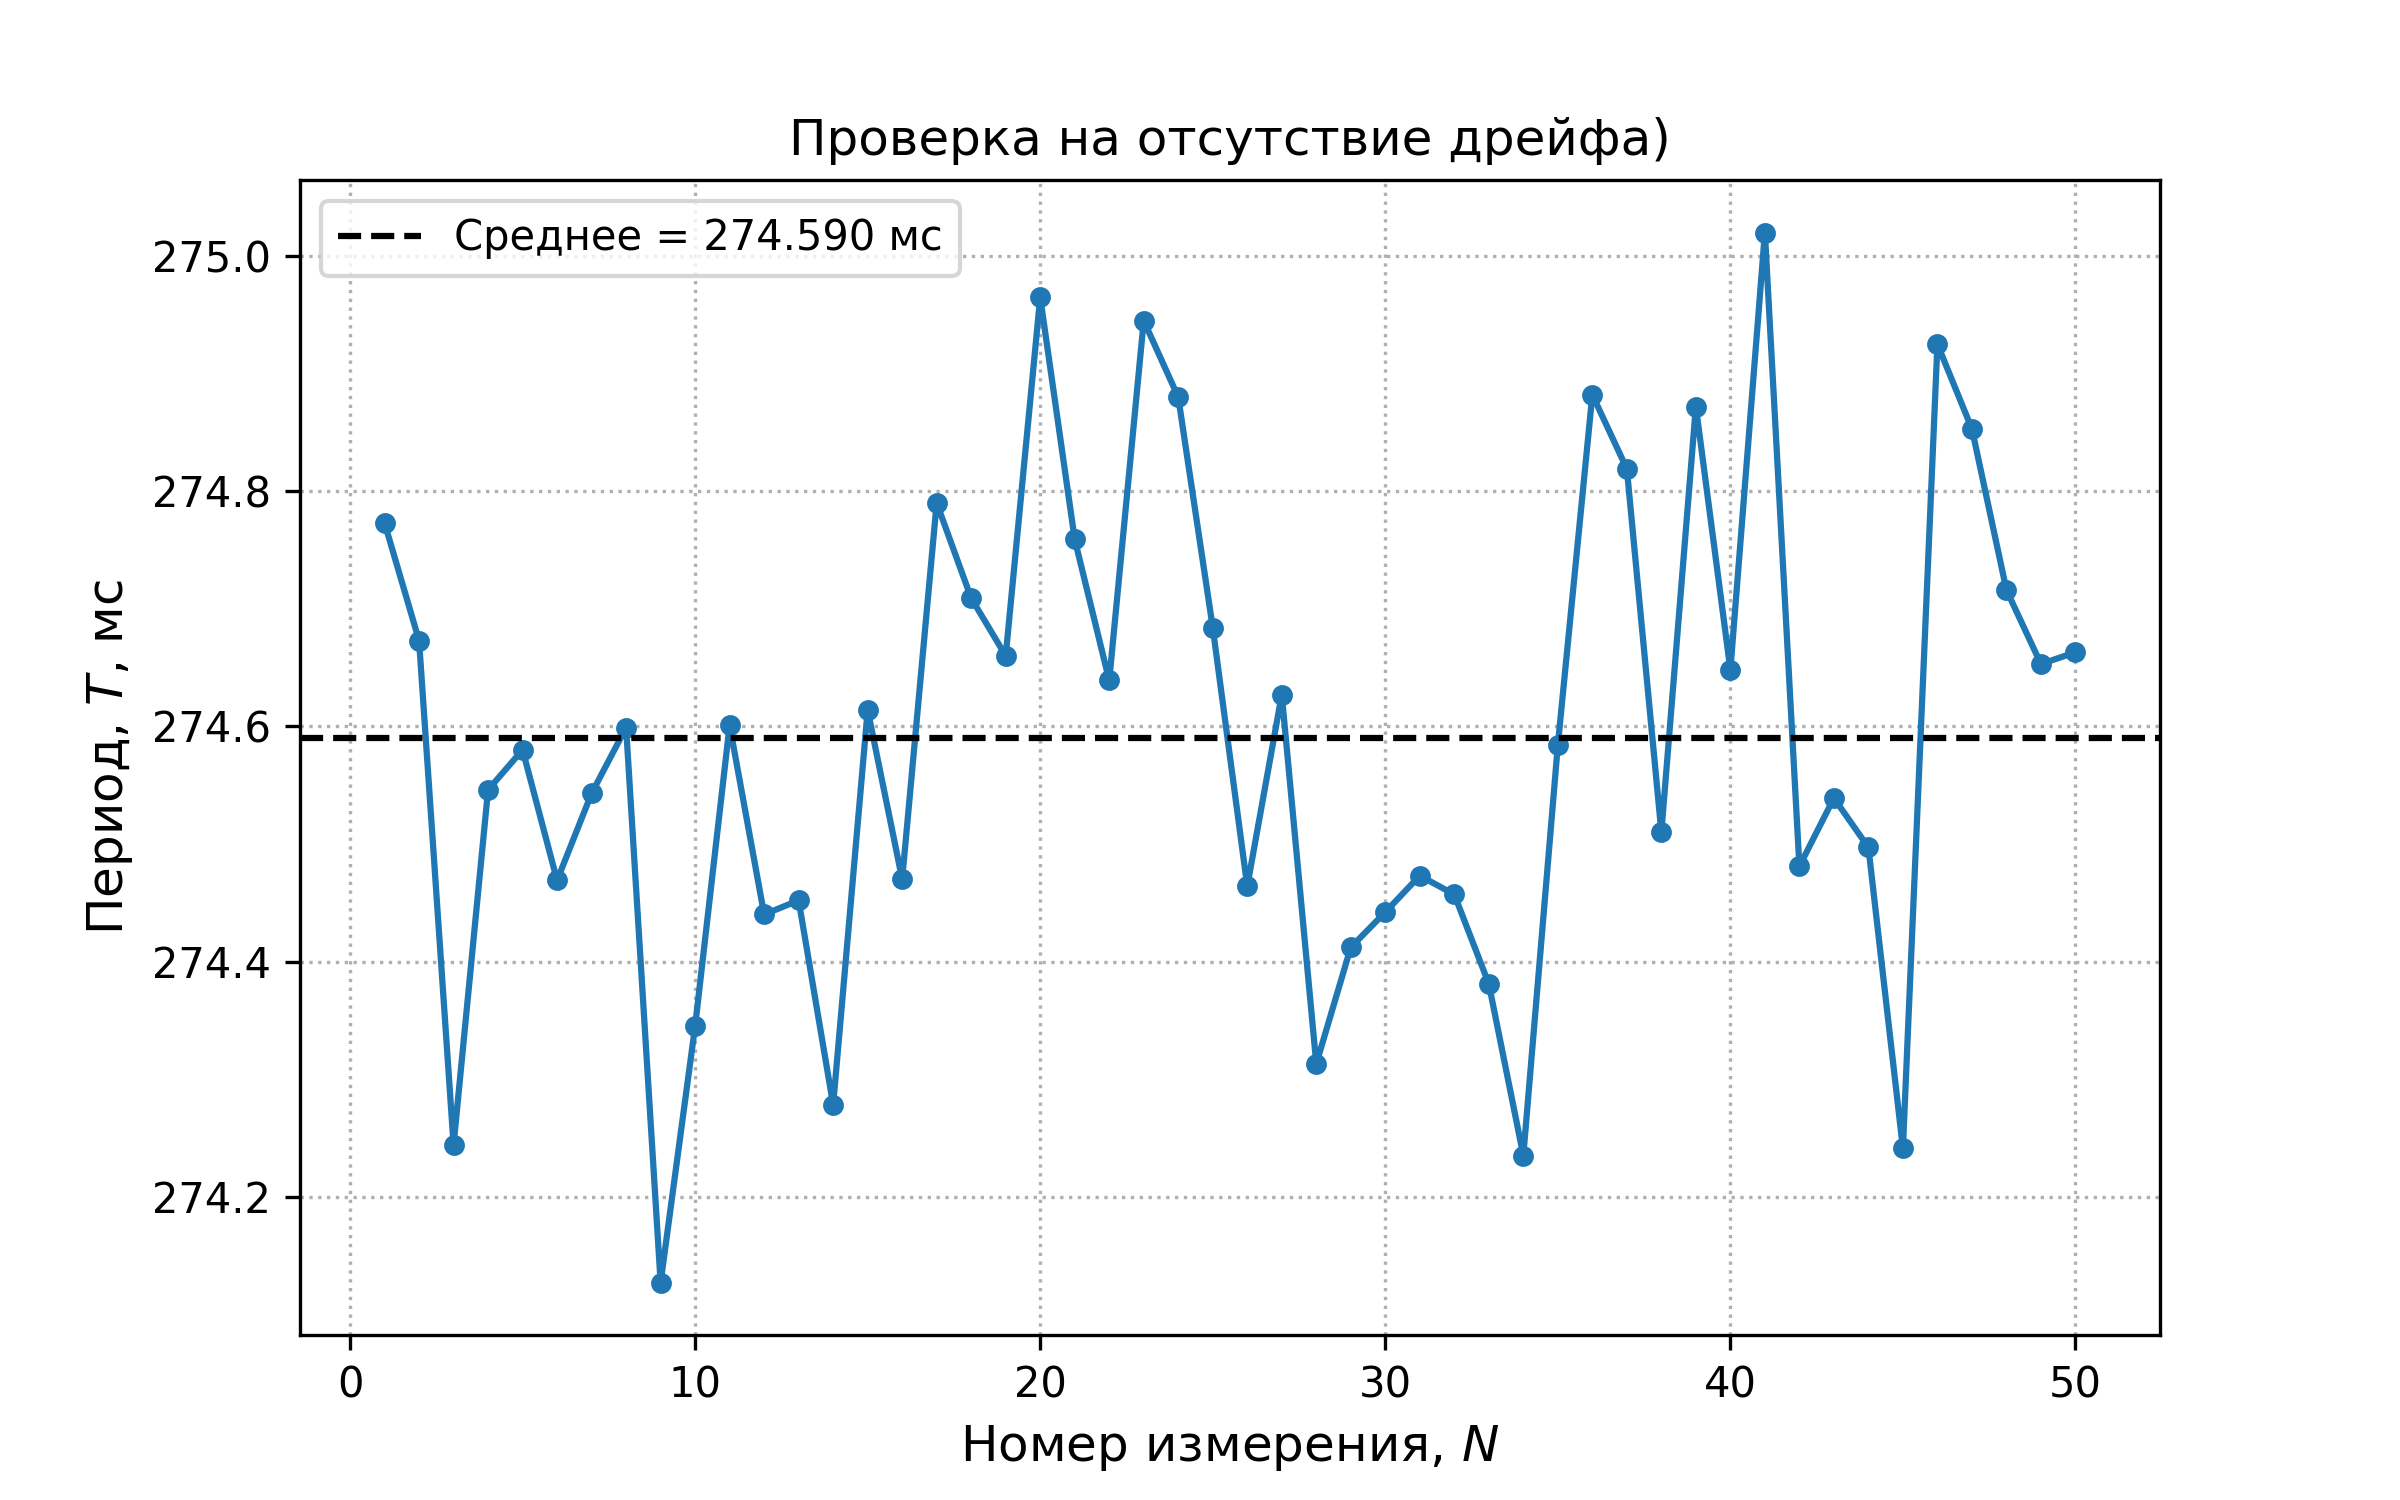
\includegraphics[width=0.8\textwidth]{drift.png}
\caption{Проверка на отсутствие временного дрейфа результатов}
\label{fig:drift}
\end{figure}

\begin{figure}[H]
\centering
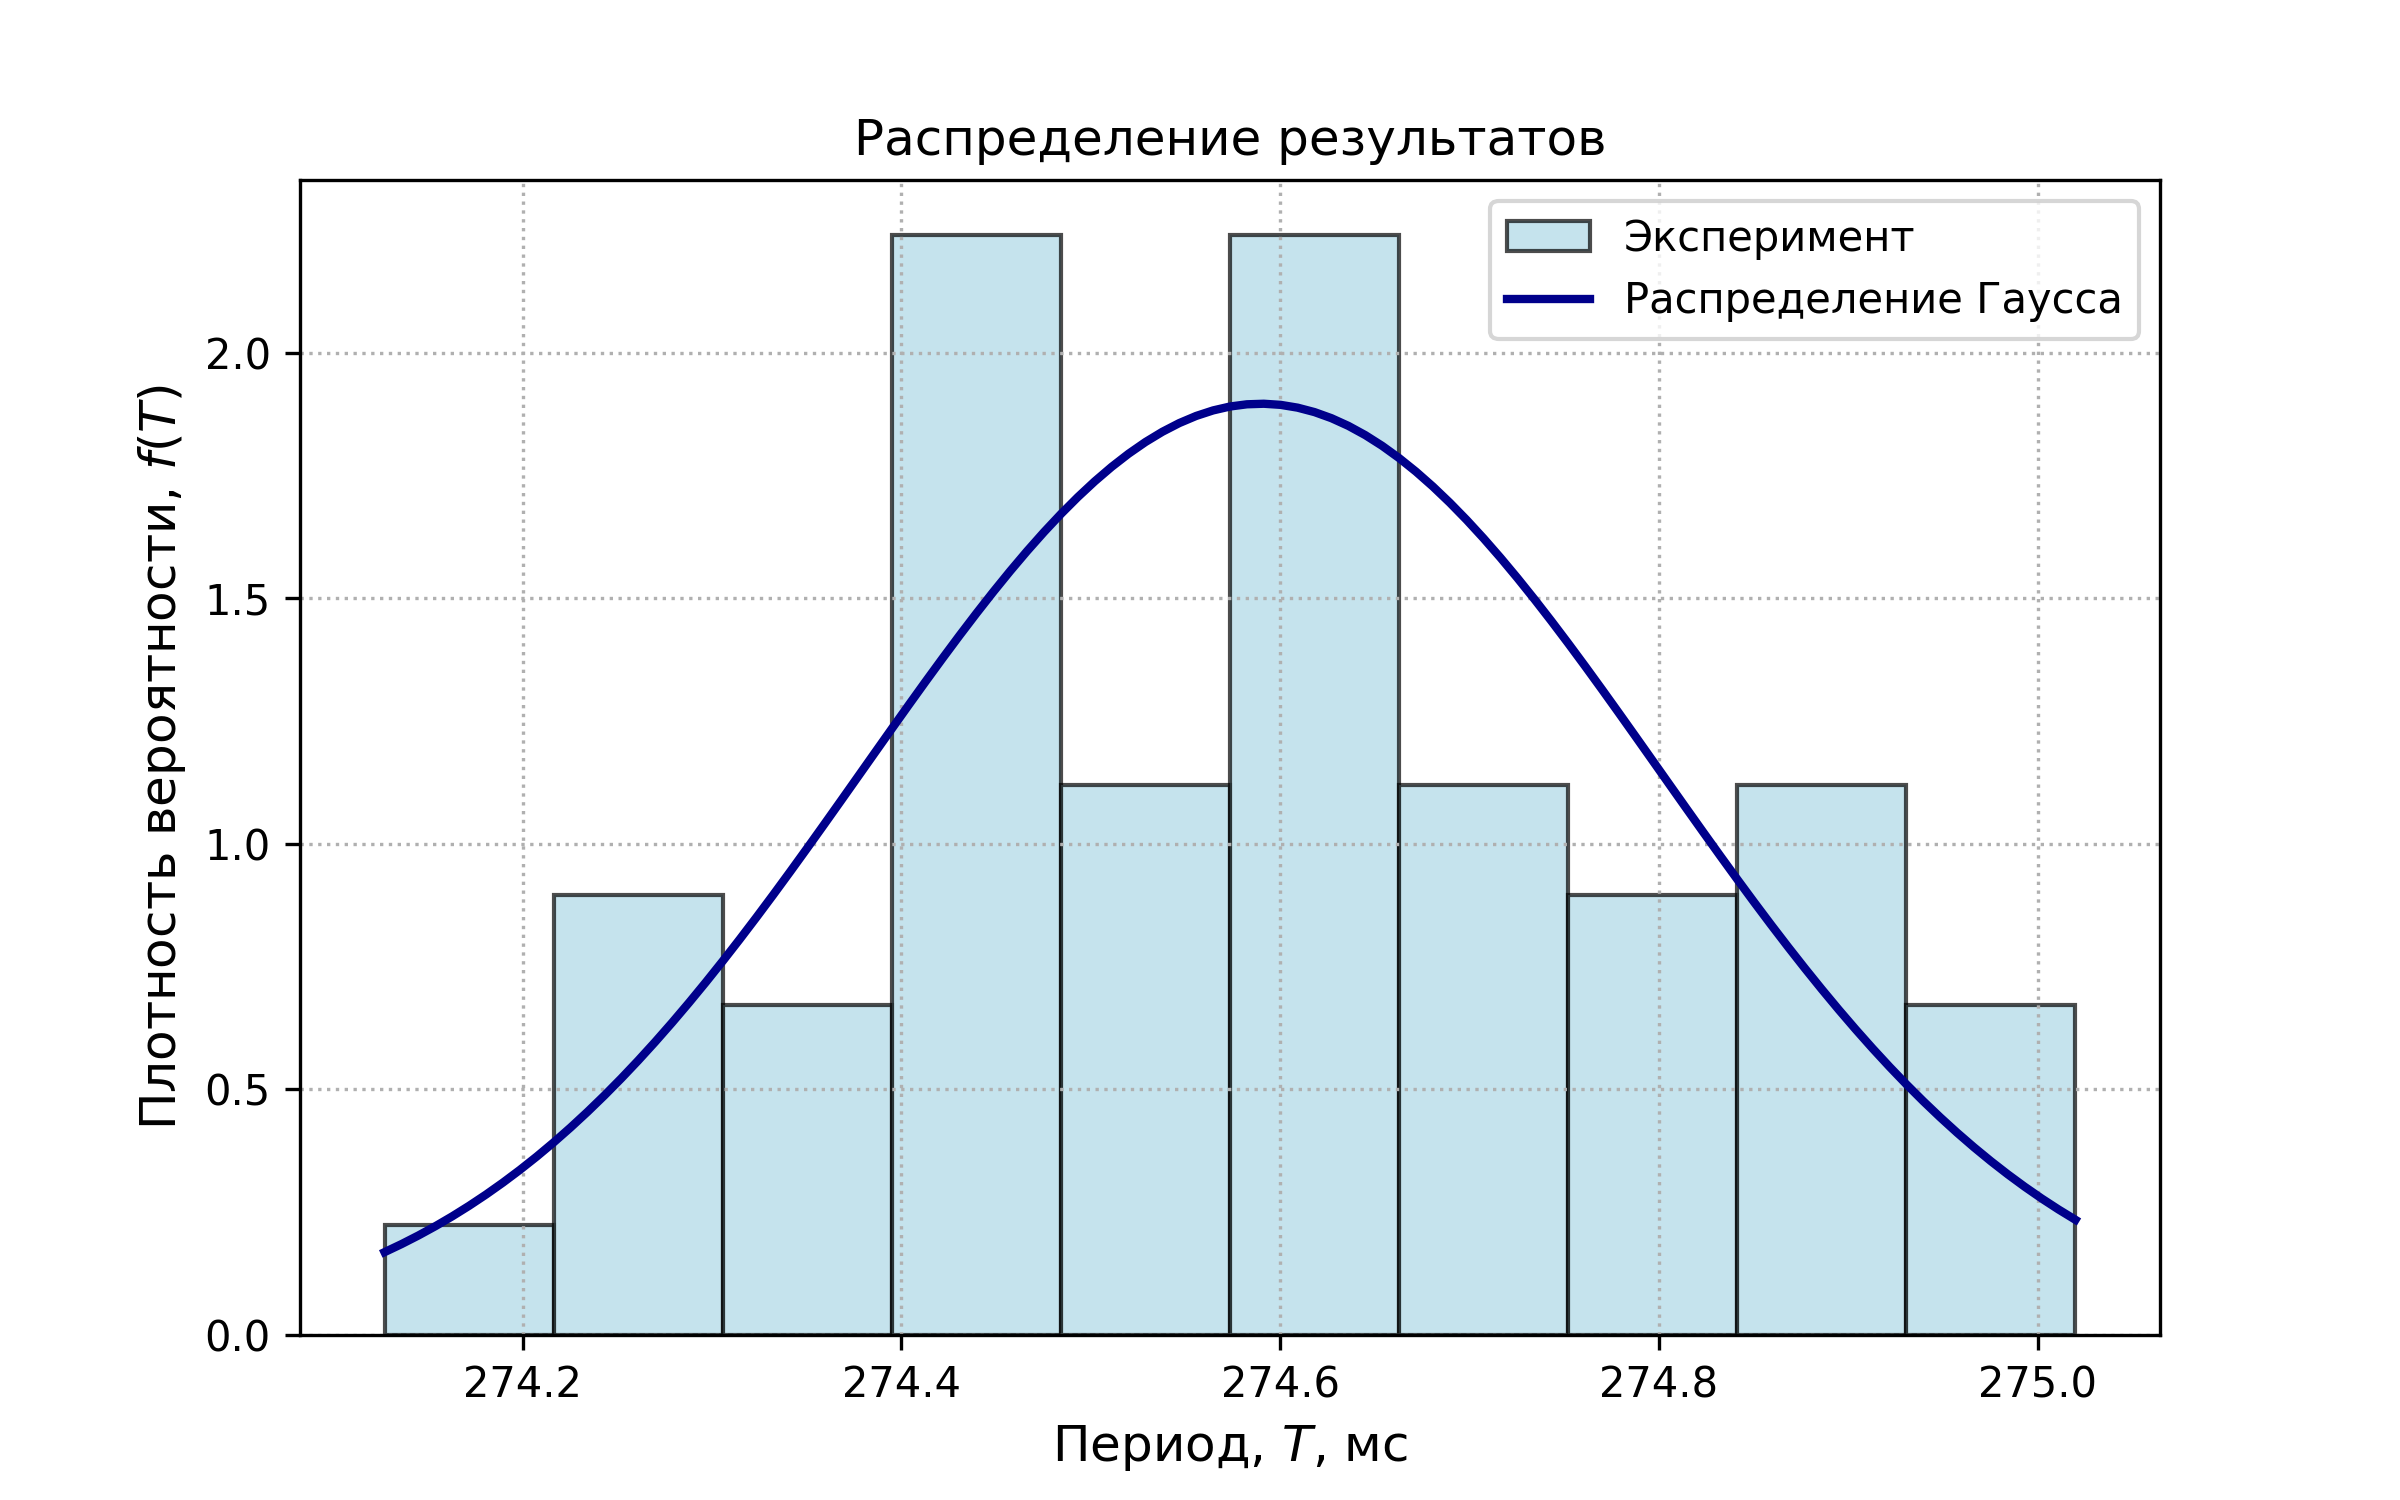
\includegraphics[width=0.8\textwidth]{hist.png}
\caption{Гистограмма распределения результатов измерений и кривая Гаусса}
\label{fig:hist}
\end{figure}

Как видно из графика на рис. \ref{fig:drift}, явного временного дрейфа (систематического увеличения или уменьшения периода) не наблюдается. Распределение результатов на рис. \ref{fig:hist} имеет колоколообразную форму, что подтверждает применимость нормального закона распределения (Гаусса) к случайным погрешностям в данном опыте.
\section{Выводы}

В ходе выполнения первой учебно-научной лабораторной работы была успешно освоена методика проведения многократных прямых измерений и их последующей статистической обработки на примере измерения периода следования импульсов с помощью электронного частотомера.

Анализ полученной выборки из 50 значений показал, что измеряемая величина не подвержена заметному временному дрейфу — процесс генерации импульсов был стационарным на протяжении всего времени снятия показаний. Построенная гистограмма распределения результатов визуально хорошо согласуется с теоретической колоколообразной кривой нормального распределения Гаусса. Это наглядно подтверждает правомерность применения классических методов математической статистики (в частности, использования коэффициентов Стьюдента) для оценки доверительных интервалов в данном физическом эксперименте.

В результате вычислений было получено наилучшее (среднее) значение периода $\bar{T} = 274.59$ мс. Главным итогом анализа погрешностей стало сравнение их вкладов в конечный результат: случайная погрешность (около $0.06$ мс) оказалась в десятки раз больше инструментальной (предел допускаемой погрешности частотомера на точной шкале составил всего $0.001$ мс). Таким образом, ситуация в опыте соответствует случаю, когда точность измерений полностью лимитируется случайными факторами (например, внутренними шумами генератора, тепловыми флуктуациями или джиттером), а не разрешающей способностью прибора.

Итоговый результат измерения периода составил $T = (274.59 \pm 0.06)$ мс. 

Прогнозируя пути повышения точности подобных экспериментов в будущем, можно сделать вывод, что простая замена измерительного прибора на более высокоточный не даст никакого существенного выигрыша. Для реального сужения доверительного интервала необходимо либо кратно увеличивать объем выборки (что позволит уменьшить случайную ошибку), либо совершенствовать саму установку.
